\section{Graphs of Functions}

\subsection{Sine}

\begin{figure}[htb]
\center
\caption{Graph of sine.}
\label{fig:graph of sine}
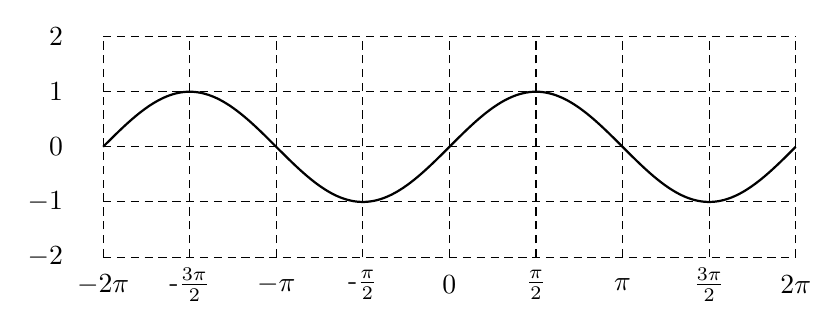
\begin{tikzpicture}[inner sep=0pt,minimum size=0mm, scale = 0.7]

\node at (3.1415, -2.5) {$\pi$};
\node at (3/2*3.1415, -2.5) {$\frac{3\pi}{2}$};
\node at (2*3.1415, -2.5) {$2\pi$};
\node at (1/2*3.1415, -2.5) {$\frac{\pi}{2}$};
\node at (0, -2.5) {$0$};
\node at (1/2*-3.1415, -2.5) {-$\frac{\pi}{2}$};
\node at (-3.1415, -2.5) {$-\pi$};
\node at (3/2*-3.1415, -2.5) {-$\frac{3\pi}{2}$};
\node at (2*-3.1415, -2.5) {$-2\pi$};

\node[left] at (-7,2) {$2$};
\node[left] at (-7,1) {$1$};
\node[left] at (-7,0) {$0$};
\node[left] at (-7,-1) {$-1$};
\node[left] at (-7,-2) {$-2$};

\draw[xstep=3.1415/2, densely dashed] (-2*3.1415,-2) grid (2*3.1415,2);
\AXES{0}{0}{2*3.1415}{2}
\draw[thick, variable = \t, domain=2*-3.1415:2*3.1415,samples=250] plot ({\t},{sin(180*\t/3.1415)});

\end{tikzpicture}
\end{figure}

Several important properties of sine can be seen by looking at a graph.  The foremost is that sine is a {\bf periodic function}, or a function that repeats itself.  This is a direct consequence of the circular nature of angles;  adding a full rotation ($2\pi$) to an angle has no effect on it, thus any angle not in the range $[0,2\pi]$ is merely an equivalent angle to one in the range.  As a result, sine has a {\bf period}, or repeat distance, of $2\pi$.\\

Another important property to note is that the sine of any angle is always in the range $[-1,1]$.  Remember that sine is the ratio of a line to its projection.  A projection can be at most the length of the line casting it, so sine can be no greater in magnitude than $1$.\\



\clearpage
\subsection{Cosine}

\begin{figure}[htb]
\center
\caption{Graph of cosine.}
\label{fig:graph of cosine}
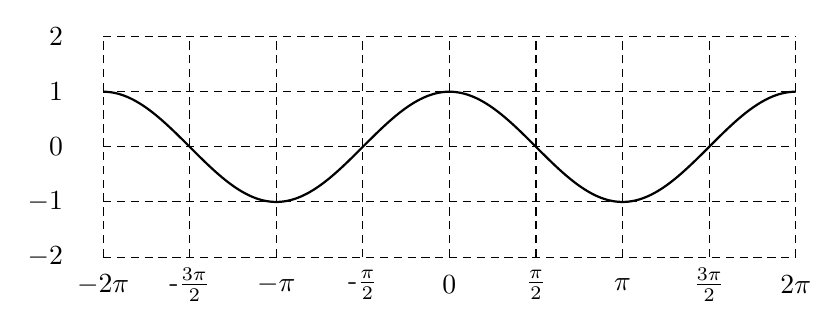
\begin{tikzpicture}[inner sep=0pt,minimum size=0mm, scale = 0.7]

\node at (3.1415, -2.5) {$\pi$};
\node at (3/2*3.1415, -2.5) {$\frac{3\pi}{2}$};
\node at (2*3.1415, -2.5) {$2\pi$};
\node at (1/2*3.1415, -2.5) {$\frac{\pi}{2}$};
\node at (0, -2.5) {$0$};
\node at (1/2*-3.1415, -2.5) {-$\frac{\pi}{2}$};
\node at (-3.1415, -2.5) {$-\pi$};
\node at (3/2*-3.1415, -2.5) {-$\frac{3\pi}{2}$};
\node at (2*-3.1415, -2.5) {$-2\pi$};

\node[left] at (-7,2) {$2$};
\node[left] at (-7,1) {$1$};
\node[left] at (-7,0) {$0$};
\node[left] at (-7,-1) {$-1$};
\node[left] at (-7,-2) {$-2$};

\draw[xstep=3.1415/2, densely dashed] (-2*3.1415,-2) grid (2*3.1415,2);
\AXES{0}{0}{2*3.1415}{2}
\draw[thick, variable = \t, domain=2*-3.1415:2*3.1415,samples=250] plot ({\t},{cos(180*\t/3.1415)});

\end{tikzpicture}
\end{figure}

There are obvious similarities between the graph of sine and the graph of cosine.  They have the same period, the same shape, and the same range.  In fact, sine and cosine are actually the same function, but with a difference in phase.  {\bf Phase} is an offset of the input of a function.  For example, if you have a function $f(x)$, $x$ is  the input variable.  $f(x+2)$ offset from $f(x)$ by a phase of $2$.\\

The phase offset for sine and cosine is $\pitwo$.  In other words $sin(x+\pitwo) = cos(x)$.  Remember, sine is a projection onto the y axis, and cosine is a projection onto the x axis.  The angle between the x and y axis is \pitwo, so it should make sense that the phase difference between sine and cosine is also \pitwo.

\begin{figure}[htb]
\center
\caption{Phase offset between sine and cosine.}
\label{fig:phase offset}
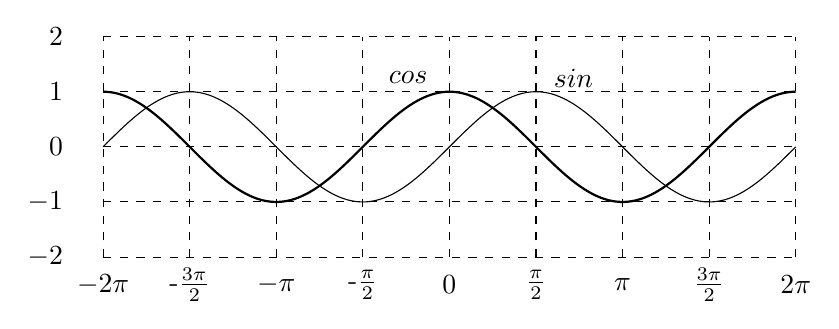
\begin{tikzpicture}[inner sep=0pt,minimum size=0mm, scale = 0.7]

\node at (3.1415, -2.5) {$\pi$};
\node at (3/2*3.1415, -2.5) {$\frac{3\pi}{2}$};
\node at (2*3.1415, -2.5) {$2\pi$};
\node at (1/2*3.1415, -2.5) {$\frac{\pi}{2}$};
\node at (0, -2.5) {$0$};
\node at (1/2*-3.1415, -2.5) {-$\frac{\pi}{2}$};
\node at (-3.1415, -2.5) {$-\pi$};
\node at (3/2*-3.1415, -2.5) {-$\frac{3\pi}{2}$};
\node at (2*-3.1415, -2.5) {$-2\pi$};

\node[left] at (-7,2) {$2$};
\node[left] at (-7,1) {$1$};
\node[left] at (-7,0) {$0$};
\node[left] at (-7,-1) {$-1$};
\node[left] at (-7,-2) {$-2$};

\draw[xstep=3.1415/2, dashed] (-2*3.1415,-2) grid (2*3.1415,2);
\AXES{0}{0}{2*3.1415}{2}
\draw[variable = \t, domain=2*-3.1415:2*3.1415,samples=250] plot ({\t},{sin(180*\t/3.1415)});
\draw[thick, variable = \t, domain=2*-3.1415:2*3.1415,samples=250] plot ({\t},{cos(180*\t/3.1415)});

\node at (2.25,1.25) {$sin$};
\node at (-.75,1.25) {$cos$};

\end{tikzpicture}
\end{figure}

\clearpage
\subsection{Tangent}


\begin{figure}[htb]
\center
\caption{Graph of tangent.}
\label{fig:graph of tan}
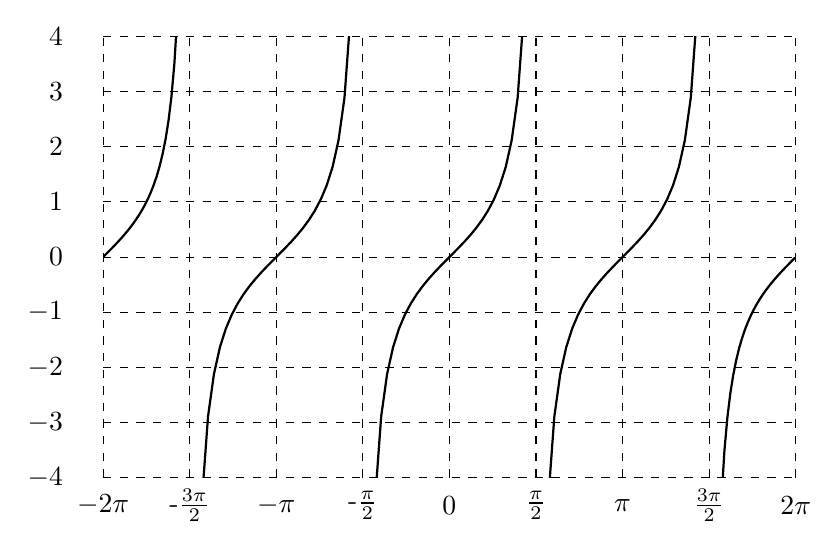
\begin{tikzpicture}[inner sep=0pt,minimum size=0mm, scale = 0.7]

\node at (3.1415, -4.5) {$\pi$};
\node at (3/2*3.1415, -4.5) {$\frac{3\pi}{2}$};
\node at (2*3.1415, -4.5) {$2\pi$};
\node at (1/2*3.1415, -4.5) {$\frac{\pi}{2}$};
\node at (0, -4.5) {$0$};
\node at (1/2*-3.1415, -4.5) {-$\frac{\pi}{2}$};
\node at (-3.1415, -4.5) {$-\pi$};
\node at (3/2*-3.1415, -4.5) {-$\frac{3\pi}{2}$};
\node at (2*-3.1415, -4.5) {$-2\pi$};

\node[left] at (-7,4) {$4$};
\node[left] at (-7,3) {$3$};
\node[left] at (-7,2) {$2$};
\node[left] at (-7,1) {$1$};
\node[left] at (-7,0) {$0$};
\node[left] at (-7,-1) {$-1$};
\node[left] at (-7,-2) {$-2$};
\node[left] at (-7,-3) {$-3$};
\node[left] at (-7,-4) {$-4$};

\draw[xstep=3.1415/2, dashed] (-2*3.1415,-4) grid (2*3.1415,4);
\AXES{0}{0}{2*3.1415}{4}

\begin{scope}
    \clip(2*-3.1415,-4) rectangle (2*3.1415,4);

\draw[thick,
 variable = \t, 
 domain=4/2*-3.1415+0.01:3/2*-3.1415-0.01,
 samples=30] 
plot ({\t},{tan(180*\t/3.1415)});


\draw[thick,
 variable = \t, 
 domain=3/2*-3.1415+0.01:1/2*-3.1415-0.01,
 samples=30] 
plot ({\t},{tan(180*\t/3.1415)});

\draw[thick,
 variable = \t, 
 domain=1/2*-3.1415+0.01:1/2*3.1415-0.01,
 samples=30] 
plot ({\t},{tan(180*\t/3.1415)});

\draw[thick,
 variable = \t, 
 domain=1/2*3.1415+0.01:3/2*3.1415-0.01,
 samples=30] 
plot ({\t},{tan(180*\t/3.1415)});

\draw[thick,
 variable = \t, 
 domain=3/2*3.1415+0.01:4/2*3.1415-0.01,
 samples=30] 
plot ({\t},{tan(180*\t/3.1415)});

\end{scope}

\end{tikzpicture}
\end{figure}

Tangent is periodic, like sine and cosine, but unlike sine and cosine it is not continuous.  A {\bf continuous function} is a function that always remains 'connected'.  You can see in the above figure that tangent has an {\bf asymptote} at \pitwo, \threepitwo, \fivepitwo, etc.  An {\bf asymptote} is a line that a function approaches, but never touches.  In this case, the asymptotes are vertical lines at \pitwo, \threepitwo, \fivepitwo, etc.  As an angle approaches \pitwo, the tangent of the angle approaches infinity from the left, and negative infinity from the right.  As a result, the tangent has a perdiod of $\pi$, a range of $(-\infty,\infty)$, and asymptotes at $\pm\frac{\pi}{2}, \pm\frac{3\pi}{2}, \pm\frac{5\pi}{2} ...$ .

\clearpage
\subsection{Secant}

\begin{figure}[htb]
\center
\caption{Graph of secant.}
\label{fig:graph of sec}
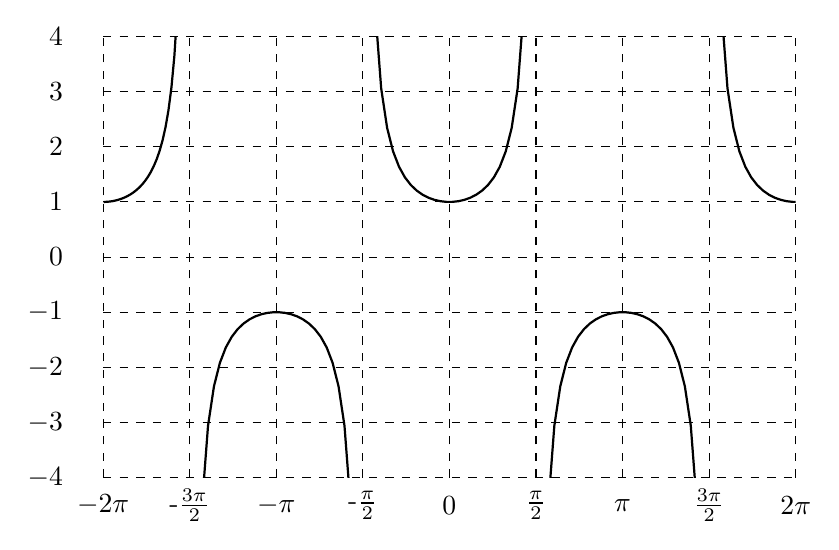
\begin{tikzpicture}[inner sep=0pt,minimum size=0mm, scale = 0.7]

\node at (3.1415, -4.5) {$\pi$};
\node at (3/2*3.1415, -4.5) {$\frac{3\pi}{2}$};
\node at (2*3.1415, -4.5) {$2\pi$};
\node at (1/2*3.1415, -4.5) {$\frac{\pi}{2}$};
\node at (0, -4.5) {$0$};
\node at (1/2*-3.1415, -4.5) {-$\frac{\pi}{2}$};
\node at (-3.1415, -4.5) {$-\pi$};
\node at (3/2*-3.1415, -4.5) {-$\frac{3\pi}{2}$};
\node at (2*-3.1415, -4.5) {$-2\pi$};

\node[left] at (-7,4) {$4$};
\node[left] at (-7,3) {$3$};
\node[left] at (-7,2) {$2$};
\node[left] at (-7,1) {$1$};
\node[left] at (-7,0) {$0$};
\node[left] at (-7,-1) {$-1$};
\node[left] at (-7,-2) {$-2$};
\node[left] at (-7,-3) {$-3$};
\node[left] at (-7,-4) {$-4$};

\draw[xstep=3.1415/2, dashed] (-2*3.1415,-4) grid (2*3.1415,4);
\AXES{0}{0}{2*3.1415}{4}

\begin{scope}
    \clip(2*-3.1415,-4) rectangle (2*3.1415,4);

\draw[thick,
 variable = \t, 
 domain=4/2*-3.1415+0.01:3/2*-3.1415-0.01,
 samples=30] 
plot ({\t},{1/cos(180*\t/3.1415)});

\draw[thick,
 variable = \t, 
 domain=3/2*-3.1415+0.01:1/2*-3.1415-0.01,
 samples=30] 
plot ({\t},{1/cos(180*\t/3.1415)});

\draw[thick,
 variable = \t, 
 domain=1/2*-3.1415+0.01:1/2*3.1415-0.01,
 samples=30] 
plot ({\t},{1/cos(180*\t/3.1415)});

\draw[thick,
 variable = \t, 
 domain=1/2*3.1415+0.01:3/2*3.1415-0.01,
 samples=30] 
plot ({\t},{1/cos(180*\t/3.1415)});

\draw[thick,
 variable = \t, 
 domain=3/2*3.1415+0.01:5/2*3.1415-0.01,
 samples=30] 
plot ({\t},{1/cos(180*\t/3.1415)});

\end{scope}

\end{tikzpicture}
\end{figure}

Secant ($\frac{1}{cos(x)}$) has a period of $2\pi$, and asymptotic at multiples of $\pm\frac{\pi}{2}, \pm\frac{3\pi}{2}, \pm\frac{5\pi}{2} ...$.  Note that secant is never in the range $(-1,1)$, so the range is $(-\infty,-1)$ and $(1,\infty)$.\\


\clearpage
\subsection{Cosecant}


\begin{figure}[htb]
\center
\caption{Graph of cosecant.}
\label{fig:graph of csc}
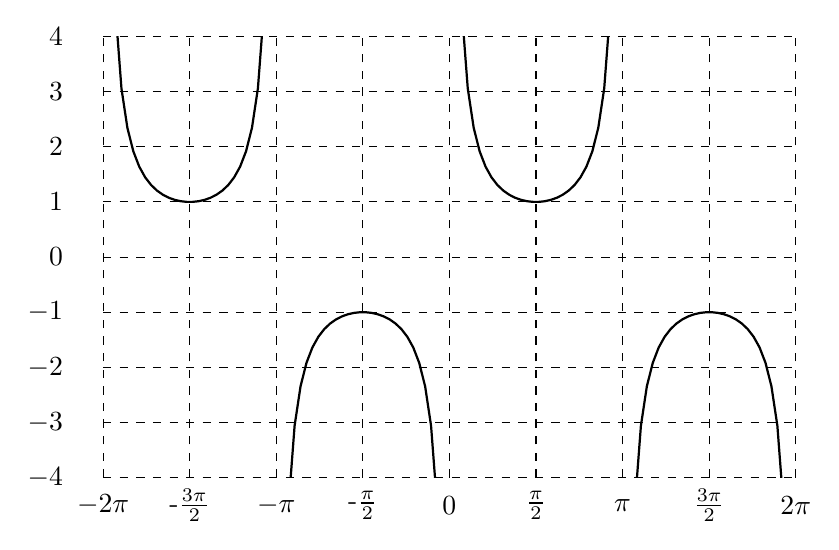
\begin{tikzpicture}[inner sep=0pt,minimum size=0mm, scale = 0.7]

\node at (3.1415, -4.5) {$\pi$};
\node at (3/2*3.1415, -4.5) {$\frac{3\pi}{2}$};
\node at (2*3.1415, -4.5) {$2\pi$};
\node at (1/2*3.1415, -4.5) {$\frac{\pi}{2}$};
\node at (0, -4.5) {$0$};
\node at (1/2*-3.1415, -4.5) {-$\frac{\pi}{2}$};
\node at (-3.1415, -4.5) {$-\pi$};
\node at (3/2*-3.1415, -4.5) {-$\frac{3\pi}{2}$};
\node at (2*-3.1415, -4.5) {$-2\pi$};

\node[left] at (-7,4) {$4$};
\node[left] at (-7,3) {$3$};
\node[left] at (-7,2) {$2$};
\node[left] at (-7,1) {$1$};
\node[left] at (-7,0) {$0$};
\node[left] at (-7,-1) {$-1$};
\node[left] at (-7,-2) {$-2$};
\node[left] at (-7,-3) {$-3$};
\node[left] at (-7,-4) {$-4$};

\draw[xstep=3.1415/2, dashed] (-2*3.1415,-4) grid (2*3.1415,4);
\AXES{0}{0}{2*3.1415}{4}

\begin{scope}
    \clip(2*-3.1415,-4) rectangle (2*3.1415,4);

\draw[thick,
 variable = \t, 
 domain=4/2*-3.1415+0.01:2/2*-3.1415-0.01,
 samples=30] 
plot ({\t},{1/sin(180*\t/3.1415)});

\draw[thick,
 variable = \t, 
 domain=2/2*-3.1415+0.01:0/2*-3.1415-0.01,
 samples=30] 
plot ({\t},{1/sin(180*\t/3.1415)});

\draw[thick,
 variable = \t, 
 domain=0/2*-3.1415+0.01:2/2*3.1415-0.01,
 samples=30] 
plot ({\t},{1/sin(180*\t/3.1415)});

\draw[thick,
 variable = \t, 
 domain=2/2*3.1415+0.01:4/2*3.1415-0.01,
 samples=30] 
plot ({\t},{1/sin(180*\t/3.1415)});

\end{scope}

\end{tikzpicture}
\end{figure}

Just as sine and cosine are the same function out of phase, secant and cosecant are the same function out of phase.  Cosecant ($\frac{1}{sin(x)}$) also has a period of $2\pi$, and a range of $(-\infty,-1)$ and $(1,\infty)$.  However, due to the phase offset of $\frac{\pi}{2}$, cosecant has asymptotes at $0, \pm\pi, \pm2\pi, \pm3\pi ...$.\\

\clearpage
\subsection{Cotangent}

\begin{figure}[htb]
\center
\caption{Graph of cotangent.}
\label{fig:graph of cot}
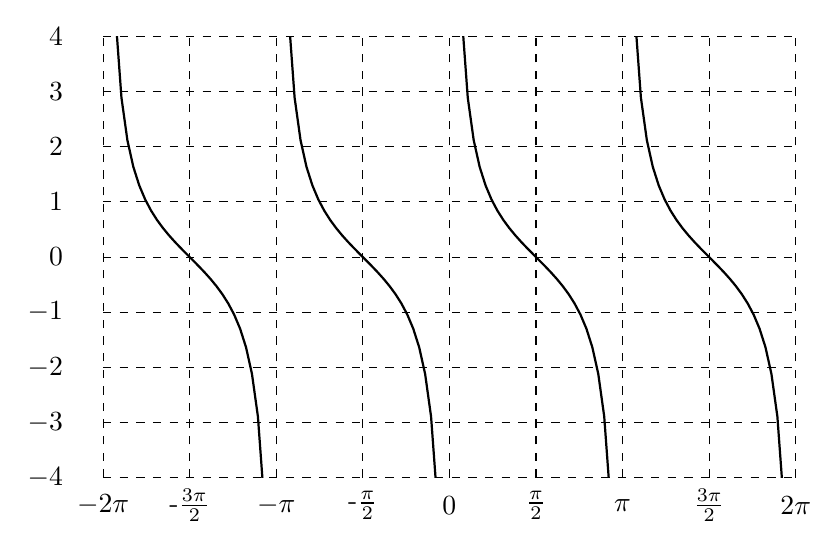
\begin{tikzpicture}[inner sep=0pt,minimum size=0mm, scale = 0.7]

\node at (3.1415, -4.5) {$\pi$};
\node at (3/2*3.1415, -4.5) {$\frac{3\pi}{2}$};
\node at (2*3.1415, -4.5) {$2\pi$};
\node at (1/2*3.1415, -4.5) {$\frac{\pi}{2}$};
\node at (0, -4.5) {$0$};
\node at (1/2*-3.1415, -4.5) {-$\frac{\pi}{2}$};
\node at (-3.1415, -4.5) {$-\pi$};
\node at (3/2*-3.1415, -4.5) {-$\frac{3\pi}{2}$};
\node at (2*-3.1415, -4.5) {$-2\pi$};

\node[left] at (-7,4) {$4$};
\node[left] at (-7,3) {$3$};
\node[left] at (-7,2) {$2$};
\node[left] at (-7,1) {$1$};
\node[left] at (-7,0) {$0$};
\node[left] at (-7,-1) {$-1$};
\node[left] at (-7,-2) {$-2$};
\node[left] at (-7,-3) {$-3$};
\node[left] at (-7,-4) {$-4$};

\draw[xstep=3.1415/2, dashed] (-2*3.1415,-4) grid (2*3.1415,4);
\AXES{0}{0}{2*3.1415}{4}

\begin{scope}
    \clip(2*-3.1415,-4) rectangle (2*3.1415,4);

\draw[thick,
 variable = \t, 
 domain=4/2*-3.1415+0.01:2/2*-3.1415-0.01,
 samples=30] 
plot ({\t},{1/tan(180*\t/3.1415)});

\draw[thick,
 variable = \t, 
 domain=2/2*-3.1415+0.01:0/2*-3.1415-0.01,
 samples=30] 
plot ({\t},{1/tan(180*\t/3.1415)});

\draw[thick,
 variable = \t, 
 domain=0/2*-3.1415+0.01:2/2*3.1415-0.01,
 samples=30] 
plot ({\t},{1/tan(180*\t/3.1415)});

\draw[thick,
 variable = \t, 
 domain=2/2*3.1415+0.01:4/2*3.1415-0.01,
 samples=30] 
plot ({\t},{1/tan(180*\t/3.1415)});
\end{scope}

\end{tikzpicture}
\end{figure}

Cotangent ($\frac{cos(x)}{sin(x)}$) is the inverse of tangent.  It also has a period of $\pi$, and a range of $(-\infty,\infty)$.  It has asymptotes at  $0, \pm\pi, \pm2\pi, \pm3\pi ...$.\\

\clearpage
\subsection{Summary}

Sine is a periodic function with a period of $2\pi$.  It oscillates between $-1$, and $1$. \\

Cosine is a phase-offset version of sine.  It is offset from sine by $\frac{\pi}{2}$.  It also has a period of $2\pi$, and a range of $[-1,1]$.\\

Tangent is a periodic function with a period of $\pi$.  Tangent has an inifinite range; $tan(\theta)$ can range from $(-\infty,\infty)$.  Tangent is a discontinuous function.  It has vertical asymptotes at $\theta = \pm \frac{\pi}{2}, \pm \frac{3\pi}{2}, \pm \frac{5\pi}{2},...$.\\

Secant is the reciprocal of cosine.  It ranges from $[1,\infty)$ and $(-\infty,1]$.  Secant is a discontinuous function, that has vertical asymptotes at $\theta = \pm \frac{\pi}{2}, \pm \frac{3\pi}{2}, \pm \frac{5\pi}{2},...$.  Secant has a period of $2\pi$.\\

Cosecant is the reciprocal of sine.  Cosecant is phase-offset from secant by $\frac{\pi}{2}$.  It has the same range as secant, and is also discontinuous, with vertical asymptotes at $\theta = 0, \pm \pi, \pm 2\pi,...$.\\

Cotangent is the reciprocal of tangent.  It also has an infinite range, and a period of $\pi$.  It is also discontinuous, with vertical asymptotes at $\theta = 0, \pm \pi, \pm 2\pi,...$.\\

\begin{figure}[htb]
\caption{Table of properties of trig. functions.}
\label{fig:table_of_properties}
\begin{center}
\begin{tabular}{|c|c|c|c|}
\hline 
function & period & range & asymptotes\\
\hline 
$sin(x)$ & $2\pi$ & $[-1,1]$ & none\\
\hline 
$cos(x)$ & $2\pi$ & $[-1,1]$ & none\\
\hline 
$tan(x)$ & $\pi$ & $[-\infty,\infty]$ & $\pm\frac{\pi}{2}, \pm\frac{3\pi}{2}, \pm\frac{5\pi}{2} ...$\\
\hline
$sec(x)$ & $2\pi$ & $(-\infty,-1)$ and $(1,\infty)$ & $\pm\frac{\pi}{2}, \pm\frac{3\pi}{2}, \pm\frac{5\pi}{2} ...$\\
\hline
$csc(x)$ & $2\pi$ & $(-\infty,-1)$ and $(1,\infty)$ & $0, \pm\pi, \pm2\pi, \pm3\pi ...$\\
\hline
$cot(x)$ & $\pi$ & $(-\infty,\infty)$ & $0, \pm\pi, \pm2\pi, \pm3\pi ...$\\
\hline
\end{tabular}
\end{center}
\end{figure}




\clearpage
\subsection{Review}

Draw and label graphs for the six trig. functions: sine, cosine, tangent, secant, cosecant, and cotangent.  Be sure to specify the range, and any asymptotes.  You should be able to draw all of these from memory, without referring back to the text.\\

